


\documentclass[10pt,a4paper]{article}

% ------------------------------------------------
% ZAKLADNI NASTAVENI A BALICKY
% ------------------------------------------------
\usepackage[T1]{fontenc}
\usepackage[utf8]{inputenc}
\usepackage[czech]{babel}
\usepackage{lmodern}
\usepackage[a4paper,margin=2.3cm,headheight=14pt]{geometry}

\usepackage{microtype}
\usepackage{graphicx}
\usepackage{float}
\usepackage{booktabs}
\usepackage{tabularx}
\usepackage{longtable}
\usepackage{array}
\usepackage{enumitem}
\usepackage{fancyhdr}
\usepackage{xcolor}
\usepackage{listings}
\usepackage{tikz}
\usepackage{multicol}
\usetikzlibrary{arrows.meta,positioning,shapes.geometric,automata}

\usepackage[hidelinks]{hyperref}

% ------------------------------------------------
% VZHLED DOKUMENTU
% ------------------------------------------------
\setlength{\parindent}{0pt}
\setlength{\parskip}{4pt}
\setlist{nosep,leftmargin=*}

\pagestyle{fancy}
\fancyhf{}
\lhead{IFJ26 -- Dokumentace projektu}
\rhead{\thepage}
\renewcommand{\headrulewidth}{0.4pt}

\hypersetup{
    pdftitle={Dokumentace projektu IFJ26},
    pdfsubject={Implementace překladače imperativního jazyka IFJ26}
}

% Sloupec s automatickým zalamováním textu
\newcolumntype{Y}{>{\raggedright\arraybackslash}X}

% ------------------------------------------------
% UDAJE K DOPLNENI
% ------------------------------------------------
\newcommand{\nazevprojektu}{Implementace překladače imperativního jazyka IFJ26}
\newcommand{\varianta}{vv-BVS}
\newcommand{\gitrepo}{https://github.com/martin-yeaaa/prekladac-ifj26}

\begin{document}

% =================================================
% TITULNI STRANA
% =================================================
\begin{titlepage}
    \centering
    {\large VYSOKÉ UČENÍ TECHNICKÉ V BRNĚ}\\[0.3cm]
    {\large Fakulta informačních technologií}\\[2.0cm]

    {\Large Dokumentace projektu}\\[0.5cm]
    {\huge\bfseries \nazevprojektu}\\[1.5cm]

    \begin{tabularx}{\textwidth}{|l|Y|Y|Y|}
        \hline
        \textbf{Člen týmu} & \textbf{VUT login} & \textbf{Osobní číslo} & \textbf{Podíl bodů} \\
        \hline
        \textbf{Martin Vaško} & \textbf{xvaskom00} & \textbf{282244} & 54 \% \\
        \hline
        Michal Bína & xbinami00 & 282028 & 13 \% \\
        \hline
        Lukáš Dvořák & xdvoral00 & 282092 & 20 \% \\
        \hline
        Jiří Švec & xsvecji00 & 281993 & 13 \% \\
        \hline
    \end{tabularx}

    \vspace{1.0cm}
    \begin{tabularx}{\textwidth}{lY}
        \textbf{Varianta zadání:} & \varianta \\
        \textbf{Implementovaná rozšíření:} &ŽÁDNÁ \\
        \textbf{Git repozitář:} & \url{\gitrepo} \\
    \end{tabularx}

    \vfill
    {\large Brno, 2026}
\end{titlepage}

\tableofcontents
\newpage

% =================================================
\section{Rozdělení práce}
% =================================================
% Uvedte, kdo se podilel na jednotlivych castech projektu.
% Pokud rozdeleni bodu neni rovnomerne, uvedte jeho duvod.

\subsection{Členové týmu a jejich odpovědnosti}

\begin{itemize}
    \item \textbf{xvaskom00:} implementace celého parseru a sémantické analýzy, tabulky symbolů a BVS, specifikace AST, nárvh a oprava gramatiky
    \item \textbf{xdvoral00:} generátor kódu 
    \item \textbf{xbinami00:} část lexeru a část gramatiky a tabulky
    \item \textbf{xsvecji00:} část lexeru a dokumentace
\end{itemize}

\subsection{Odůvodnění rozdělení bodů}
DOPLŇTE VLASTNÍ TEXT.

% =================================================
\section{Spolupráce a vývoj}
% =================================================
\subsection{Organizace spolupráce a verzování}
Jako komunikační prostředek byl zvolen \texttt{Discord}. Neukázal se však jako dostačující, protože někteří členové týmu na zprávy reagovali později, než bylo potřeba.

Důležité věci se probraly na 2 offline schůzkách a 2 online schůzkách.

Pro verzování byl využit \texttt{github}. 



\subsection{Code review a schvalování změn}
DOPLŇTE VLASTNÍ TEXT.

\subsection{Testování}
DOPLŇTE VLASTNÍ TEXT.

\subsection{Formátování zdrojového kódu}
K formátování zdrojového kódu byl využit \texttt{clang-format}.

% =================================================
\section{Architektura řešení}
% =================================================
% Vlozte vlastni blokove schema. Diagram musi ukazovat moduly,
% datove toky a struktury predavane mezi moduly.

\subsection{Blokové schéma}

% Moznost vlozeni externiho obrazku:
% \begin{figure}[H]
%     \centering
%     \includegraphics[width=\textwidth]{architektura.pdf}
%     \caption{Blokové schéma architektury překladače}
%     \label{fig:architektura}
% \end{figure}

% Nebo vytvorte diagram primo v TikZ:
\begin{figure}[H]
    \centering
    \fbox{\parbox[c][5cm][c]{0.9\textwidth}{
        \centering
        ZDE VLOŽTE BLOKOVÉ SCHÉMA ARCHITEKTURY
    }}
    \caption{Blokové schéma architektury překladače}
    \label{fig:architektura}
\end{figure}

\subsection{Popis datových toků a komponent}
DOPLŇTE VLASTNÍ TEXT.

% =================================================
\section{Lexikální analýza}
% =================================================
\subsection{Konečný automat}
% Vlozte vlastni diagram automatu, napr. jako PDF/PNG,
% nebo jej vytvorte pomoci TikZ.

\begin{figure}[H]
    \centering
    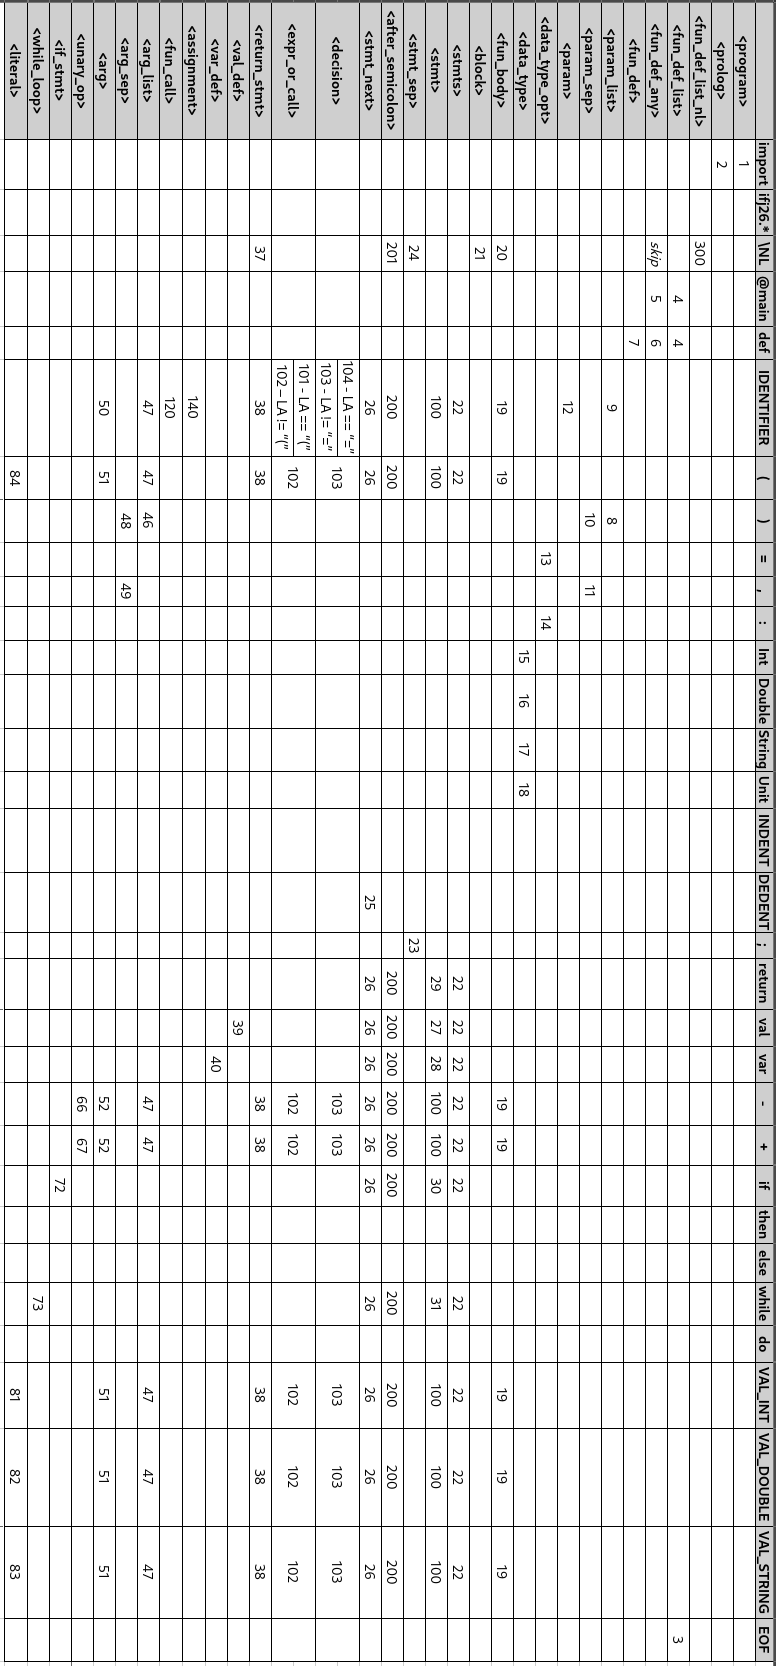
\includegraphics[
        width=\textwidth,
        height=0.75\textheight,
        keepaspectratio
    ]{LL tabulka.png}
    \caption{Konečný automat lexikálního analyzátoru}
    \label{fig:automat}
\end{figure}

\subsection{Odchylky od standardního modelu}
1. Token pro \texttt{@} byl nakonec řešen jinak (jako celek \texttt{@main)}. \\
2. Mezery, \texttt{LF} a \texttt{EOF} mají vlastní pravidla. \\
3. Diagram dovoluje pouze jedno podtržítko mezi číslicemi, ale implementace dovoluje více. \\
4. Vnořené komentáře jsou řešeny složitěji a v diagramu by šly těžko zapsat.

% =================================================
\section{Syntaktická analýza}
% =================================================
\subsection{LL gramatika}
% ZDE VLOZTE VLASTNI GRAMATIKU.

1 <program> $\to$ <prolog> <fun\_def\_list\_nl> \\
2 <prolog> $\to$ import ifj26.* \\
300 <fun\_def\_list\_nl> $\to$ \textbackslash NL <fun\_def\_list> EOF \\
3 <fun\_def\_list> $\to$ epsilon \\
4 <fun\_def\_list> $\to$ <fun\_def\_any> <fun\_def\_list\_nl>\\
5 <fun\_def\_any> $\to$ @main <fun\_def> \\
- POZOR: parser ve pravidle 5 ignoruje \textbackslash NL 
mezi @main a <fun\_def>, i když lexer \textbackslash NL, 
vydá, protože lexer porušil dohodu vypisovat pouze povinné nebo zakázané \textbackslash NL

6 <fun\_def\_any> $\to$ <fun\_def>\\
7 <fun\_def> $\to$ def IDENTIFIER (<param\_list>) <data\_type\_opt> = <fun\_body>\\
8 <param\_list> $\to$ epsilon\\
9 <param\_list> $\to$ <param> <param\_sep>\\
10 <param\_sep> $\to$ epsilon\\
11 <param\_sep> $\to$ , <param> <param\_sep>\\
12 <param> $\to$ IDENTIFIER : <data\_type>\\
13 <data\_type\_opt> $\to$ epsilon\\
14 <data\_type\_opt> $\to$ : <data\_type>\\
15 <data\_type> $\to$ Int\\
16 <data\_type> $\to$ Double\\
17 <data\_type> $\to$ String\\
18 <data\_type> $\to$ Unit\\
19 <fun\_body> $\to$ <expr\_or\_call>\\
20 <fun\_body> $\to$ <block>\\
21 <block> $\to$ \textbackslash NL INDENT <stmts> DEDENT  + "VYTVORI" UMELY TOKEN \textbackslash NL\\
22 <stmts> $\to$ <stmt> <stmt\_sep>\\
23 <stmt\_sep> $\to$ ; <after\_semicolon>\\
24 <stmt\_sep> $\to$ \textbackslash NL <stmt\_next>\\
200 <after\_semicolon> $\to$ <stmts>\\
201 <after\_semicolon> $\to$ \textbackslash NL <stmt\_next>\\
25 <stmt\_next> $\to$ epsilon\\
26 <stmt\_next> $\to$ <stmts>\\
27 <stmt> $\to$ <val\_def>\\
28 <stmt> $\to$ <var\_def>\\
29 <stmt> $\to$ return <return\_stmt>\\
30 <stmt> $\to$ <if\_stmt>\\
31 <stmt> $\to$ <while\_loop>\\
100 <stmt> $\to$ <decision>\\

VYUŽÍVÁ LOOK AHEAD, pokud zpracovávaný token je IDENTIFIER\\
101 <expr\_or\_call> $\to$ <fun\_call>   \hspace{0.7cm}   Pokud look ahead je (\\
102 <expr\_or\_call> $\to$ <expr>   \hspace{0.7cm}   Pokud look ahead není (\\

VYUŽÍVÁ LOOK AHEAD, pokud zpracovávaný token je IDENTIFIER\\
103 <decision> $\to$ <expr\_or\_call> \hspace{0.7cm}  Pokud look ahead není =\\
104 <decision> $\to$ <assignment> \hspace{0.7cm}  Pokud look ahead je =\\
\\
\\

120 <fun\_call> $\to$ IDENTIFIER(<arg\_list>)\\
140 <assignment> $\to$ IDENTIFIER = <expr\_or\_call>\\

37 <return\_stmt> $\to$ epsilon\\
38 <return\_stmt> $\to$ <expr\_or\_call>\\
39 <val\_def> $\to$ val IDENTIFIER <data\_type\_opt> = <expr\_or\_call>\\
40 <var\_def> $\to$ var IDENTIFIER <data\_type\_opt> = <expr\_or\_call>\\

46 <arg\_list> $\to$ epsilon\\
47 <arg\_list> $\to$ <arg> <arg\_sep>\\
48 <arg\_sep> $\to$ epsilon\\
49 <arg\_sep> $\to$ , <arg> <arg\_sep>\\
50 <arg> $\to$ IDENTIFIER\\
51 <arg> $\to$ <literal>\\
52 <arg> $\to$ <unary\_op> <literal>\\

66 <unary\_op> $\to$ -\\
67 <unary\_op> $\to$ +\\

72 <if\_stmt> $\to$ if <cond> then <block> \textbackslash NL else <block>\\
73 <while\_loop> $\to$ while <cond> do <block>\\

81 <literal> $\to$ VAL\_INT\\
82 <literal> $\to$ VAL\_DOUBLE\\
83 <literal> $\to$ VAL\_STRING\\
84 <literal> $\to$ ()\\

\textbackslash NL je token nového řádku pouze tam, kde jsou nové řádky
 vyžadovány nebo zakázány.\\
<expr> a <cond> se řeší pomocí precedenční syntaktické analýzy.\\
Pravidla jsou nepravidelně očíslovaná, protože původní očíslovaná pravidla obsahovala
chyby. Hodně pravidel bylo odstraněno a novým pravidlům jsme přidělili velká čísla,
aby se nepřekrývala se starými.

\subsection{LL tabulka}

\begin{figure}[H]
    \centering
    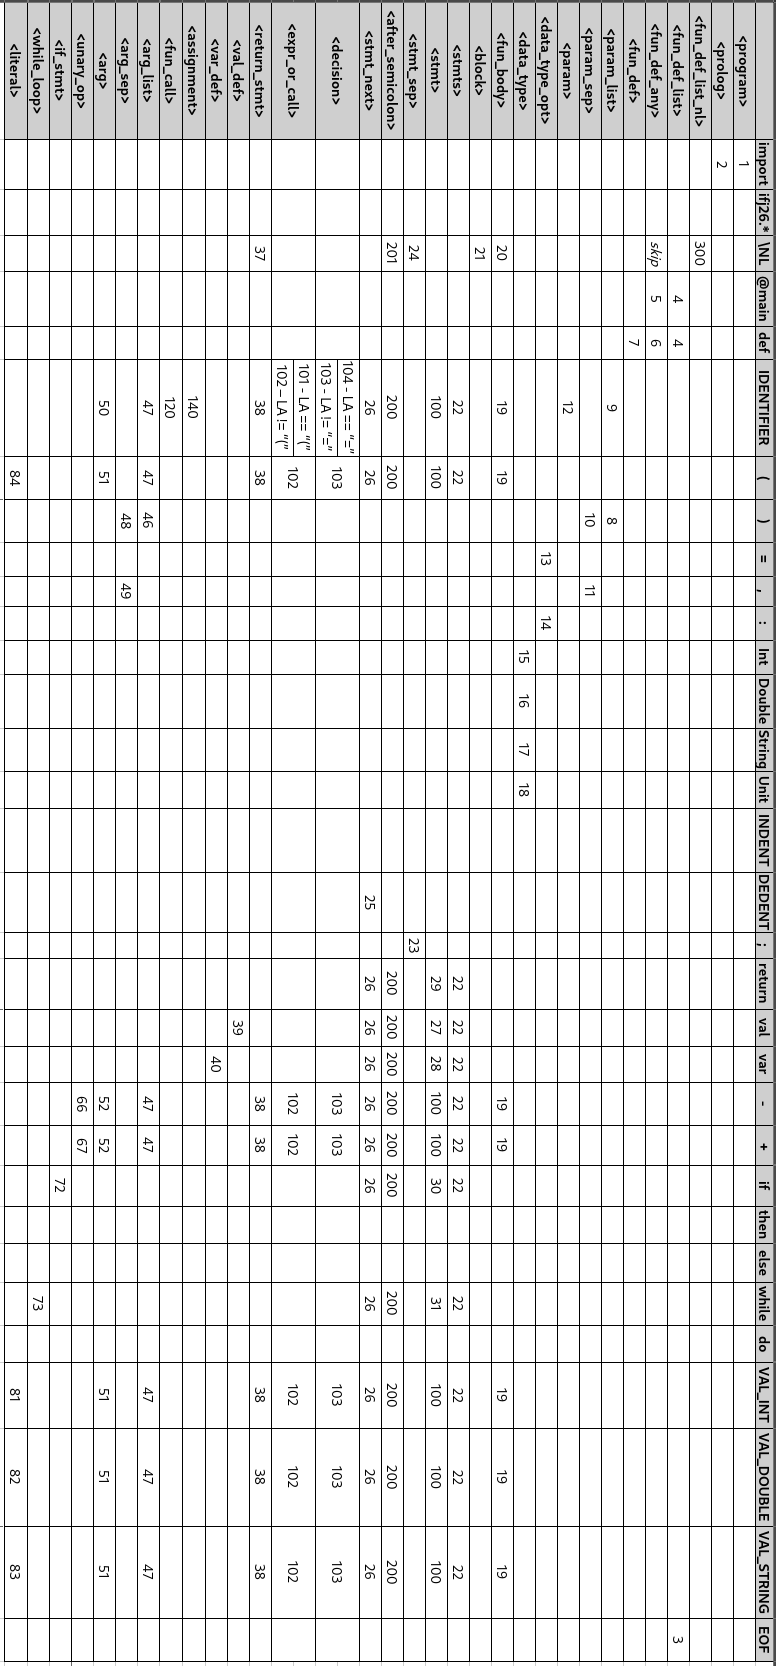
\includegraphics[
        width=\textwidth,
        height=0.89\textheight,
        keepaspectratio
    ]{LL tabulka.png}
    \label{fig:LL tabulka}
\end{figure}

Vysvětlivky: \\
skip – právě analyzovaný token se přeskočí, přečte se další \\
LA – look-ahead token, tedy token následující po právě analyzovaném tokenu\\

\subsection{Redukční pravidla precedenční syntaktické analýzy}

\begin{multicols}{2}
E $\to$ i \\
E $\to$ VAL\_STRING \\
E $\to$ VAL\_INT \\
E $\to$ VAL\_DOUBLE \\
E $\to$ () \hspace{0.7cm} (Literál Unit!) \\
E $\to$ +E \\
E $\to$ -E \\
E $\to$ E+E \\
E $\to$ E-E \\
E $\to$ E*E \\
E $\to$ E/E \\
E $\to$ (E) \\
E $\to$ E > E \\
E $\to$ E >= E \\
E $\to$ E < E \\
E $\to$ E <= E \\
E $\to$ E == E \\
E $\to$ E != E 
\end{multicols}

Vysvětlivky: \\
i – identifikátor \\
VAL\_STRING, VAL\_INT, VAL\_DOUBLE – Literály daných typů\\
E ve značení LL gramatiky je výraz reprezentovaný neterminálem
 <expr> nebo <cond>.


\subsection{Precedenční tabulka}

\begin{figure}[H]
    \centering
    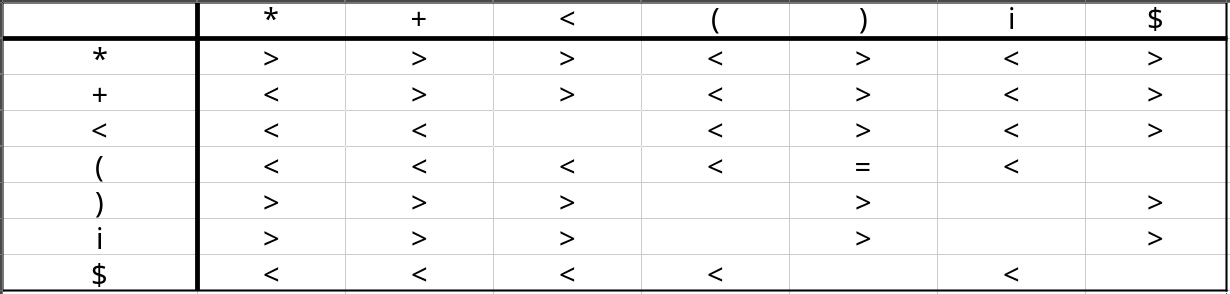
\includegraphics[
        width=\textwidth,
        height=0.89\textheight,
        keepaspectratio
    ]{Precedencni tabulka.png}
    \label{fig:Precedencni tabulka}
\end{figure}

V tabulce nejsou zobrazeny všechny operátory, protože operátory se stejnou prioritou mají 
naprosto identické řádky i sloupce. Vytvořili jsme z nich skupiny a do tabulky vložili pouze
jeden operátor reprezentující celou skupinu.

\textbf{*} reprezentuje *  / \\
\textbf{+} reprezentuje + - \\
\textbf{<} reprezentuje < <= > >= == != \\
\textbf{(} reprezentuje pouze sebe \\
\textbf{)} reprezentuje pouze sebe \\
\textbf{i} reprezentuje identifikátory a literály \\
\textbf{\$} na zásobníku je speciální znak, který se chová jako terminál a je vždy na spodku zásobníku.\\
\textbf{\$} na vstupu je ukončovač výrazu.

% =================================================
\section{Popis implementovaných modulů}
% =================================================
% Pro kazdou dvojici .c/.h uvedte kratky, vecny popis.
% Radky podle potreby pridejte nebo odeberte.

\begin{longtable}{p{0.30\textwidth}p{0.68\textwidth}}
    \toprule
    \textbf{Modul} & \textbf{Stručný popis odpovědnosti modulu} \\
    \midrule
    \texttt{main.c} & Vstupní bod celého programu. \\
    \texttt{lexer.c/.h} & Ze zdrojového kódu v jazyce \texttt{IFJ26}, který si
     celý předem zanalyzuje, umožnuje postupně vrátit všechny vytvořené tokeny
      z programu.  \\
    \texttt{parser.c/.h/\_priv.h} & Volá funkce všech hlavních modulů potřebných
     pro překlad, zpracovává tokeny pomocí syntaktické analýzy založené na 
     LL gramatice metodou rekurzivního sestupu (kromě tokenů výrazů) a zároveň 
     při tom vytváří abstraktní syntaktický strom. \\
    \texttt{expr\_parser.c/.h/\_priv.h} & Zpracovává tokeny všech výrazů pouze pomocí
     precedenční syntaktické analýzy, a zároveň při tom vytváří abstraktní 
     syntaktický strom. \\
    \texttt{ast\_module.c/.h} & Obsahuje funkce pro tvorbu abstraktního
     syntaktického stromu (AST). \\
    \texttt{semantics.c/.h/\_priv.h} & Z BST kontroluje, zda je program 
     sémanticky správně a vrací abstraktní sémantický strom.\\
    \texttt{symtable.c / symtable.h} & DOPLŇTE \\
    \texttt{bst.c / bst.h / bst\_priv.h} & Implementace výškově vyváženého 
    binárního vyhledávacího stromu. Je implementován jako AVL strom, klíčem 
    je řetězec. \\
    \texttt{codegen.c / codegen.h} & DOPLŇTE \\
     
    \texttt{error\_codes.h} & Obsahuje definice konstant chybových 
    návratových kódů a makro pro vypisování chybových hlášek. \\
     
    \bottomrule
\end{longtable}



% =================================================
\section{Použité zdroje}
% =================================================
% Uvedte bibliograficke citace vsech prevzatych zdroju,
% vcetne kodu a algoritmu. Zvolte jednotny citacni format.

\begin{enumerate}
    \item DOPLŇTE BIBLIOGRAFICKOU CITACI.
    \item DOPLŇTE BIBLIOGRAFICKOU CITACI.
\end{enumerate}

% =================================================
\section{Využití nástrojů AI}
% =================================================
% Podle zadani uvedte konkretni nastroje a modely, typicky postup,
% problemy a priklady navrhu, ktere jste nevyuzili nebo upravili.
% Tuto cast vyplnte vlastnimi skutecnymi zkusenostmi.

\subsection{Použité nástroje a modely}
ChatGPT byl použit k dovysvětlení zadání a funkci dílčích částí překladače, k vyplnění jednoduchých polí podle předlohy a ke konzultaci našeho řešení. \\
Dále byl využit k tvorbě šablony pro tuto dokumentaci.

\subsection{Pracovní postup}
DOPLŇTE VLASTNÍ TEXT.

\subsection{Problémy a nevyužité nebo upravené návrhy}
DOPLŇTE VLASTNÍ TEXT.

\end{document}




